% Paper template for TAR 2022
% (C) 2014 Jan Šnajder, Goran Glavaš, Domagoj Alagić, Mladen Karan
% TakeLab, FER

\documentclass[10pt, a4paper]{article}

\usepackage{tar2023}

\usepackage[utf8]{inputenc}
\usepackage[pdftex]{graphicx}
\usepackage{booktabs}
\usepackage{amsmath}
\usepackage{amssymb}
\usepackage{multirow}
\usepackage{cleveref}
\usepackage{float}

\title{Transformers, do we really need them for detecting stress?}

\name{Sven Šćekić, Marko Kuzmić, Lovro Bučar}

\address{
    University of Zagreb, Faculty of Electrical Engineering and Computing\\
    Unska 3, 10000 Zagreb, Croatia\\
    \texttt{\{sven.scekic, marko.kuzmic, lovro.bucar\}@fer.hr}\\
}


\abstract{
    In the modern day and age, where negative emotions such as stress are present in everyday life of most people, social media allows them to share those emotions with the world.
    Using posts from the social media site Reddit, the dataset Dreaddit was created.
    In this paper we will explore different approaches for stress detection using some simple and some more advanced models.
    Models that we worked with were logistic regression along with two transformer approaches: DistilBERT and Chat GPT 3.5 Turbo.
    Our goal was to compare these different approaches to stress detection and find out which model would produce the best results while also not being too expensive and complex.
}

\begin{document}

\maketitleabstract

\section{Introduction}

Stress is a very common feeling everyone experiences in a smaller or larger amount during their life.
It negatively impacts our health and detecting it could enable us to help the person who is experiencing it and improve their existing situation.
This paper will try to find the optimal approach of detecting stressful situations from user descriptions.
For this task we will be using the Dreaddit dataset~\citep{turcan-mckeown-2019-dreaddit} which contains user posts from the Reddit website.
Throughout this paper we will be referencing the original one where the dataset was introduced.
\hfill \break
\hfill \break
In the first part of the paper we are going to describe the dataset, followed by the models that we decided to use to tackle the problem.
We tried to continue the research of the authors of the dataset and use their best performing model to compare it with some other currently popular solutions.
In the end we are going to try to answer the question if the more complex and costly solutions were really justified or should this problem be solved with a more simple approach.

\section{Related Work}
Stress detection was researched in a couple of other approaches in the last couple of years.
One of the approaches was detecting stress using deep neural networks and psychological signals~\citep{stress-neural}.
This work however focused more on the medical aspects of stress while our aim was to detect stress using persons description of an event.
The approach that we looked at the most was by the authors of the dataset~\citep{turcan-mckeown-2019-dreaddit}.
They focused on developing the dataset as well as testing how different models solved the given task.

\section{Dataset}

The dataset that is used in this paper was introduced in a paper which collected posts from a webside Reddit~\citep{turcan-mckeown-2019-dreaddit}.
On that website users can create posts in communities which focus on specific topics called subreddits.
\hfill \break
\hfill \break
\hfill \break
The dataset consists of posts from subreddits where stressful topics are likely to be discussed in between January 1, 2017 and November 19, 2018.
These subreddits fall into one of these categories:

\begin{itemize}
    \item \textbf{Social}: The posts from this category are from the subreddit called \verb|r/relationships|.
        Posts from this subreddit talk about problems in relationships, romantic or non-romantic.
    \item \textbf{Abuse}: posts from this category describe topics related to abuse in relationships and users share their experiences and advices.
        Subreddits that fall into this category are \verb|r/domesticviolence| and \verb|r/survivorofabuse|.
    \item \textbf{Anxiety}: subreddits from this category are \verb|r/anxiety| and \verb|r/stress|.
        Users in posts from this category talk about these mental illnesses, their symptoms, share advices and stories regarding these illnesses.
    \item \textbf{PTSD}: Same as the Anxiety category, posts from this category talk about mental illness, but focus on Post-Traumatic Stress Disorder.
        The only subreddit from this category is \verb|r/ptsd| and same as with posts from the Anxiety category, users share advices and stories and ask questions about the illness.
    \item \textbf{Financial}: posts from subreddits that fall into this category talk about difficult financial situations, share stories about homelessness and other stressful financial topics.
        Subreddits from this category are \verb|r/almosthomeless|, \verb|r/assistance|, \verb|r/food_pantry| and \verb|r/homeless|.
\end{itemize}

In the dataset there are 187,444 posts in total from these 10 subreddits.
The distribution of these posts can be seen in the Table~\ref{tab:dataset-distribution}.

\begin{table*}
    \caption{Distribution of collected posts}
    \label{tab:dataset-distribution}
    \begin{center}
        \begin{tabular}{|l|l|r|r|r|}
            \hline
            \textbf{Topic} & \textbf{Subreddit Name} & \textbf{Total Posts} & \textbf{Avg Tokens/Post} & \textbf{Labeled Segments}\\
            \hline
            Social                     & r/relationships    & 107,908 & 578 & 694 \\ \hline
            \multirow{2}{*}{Abuse}     & r/domesticviolence & 1,529   & 365 & 388 \\
                                       & r/survivorsofabuse & 1,372   & 444 & 315 \\ \hline
            \multirow{2}{*}{Anxiety}   & r/anxiety          & 58,130  & 193 & 650 \\
                                       & r/stress           & 1,078   & 107 & 78  \\ \hline
            PTSD                       & r/ptsd             & 4,910   & 265 & 711 \\ \hline
            \multirow{4}{*}{Financial} & r/almosthomeless   & 547     & 261 & 99  \\
                                       & r/assistance       & 9,243   & 209 & 355 \\
                                       & r/food\_pantry     & 343     & 187 & 43  \\
                                       & r/homeless         & 2,384   & 143 & 220 \\ \hline
        \end{tabular}
    \end{center}
\end{table*}


\hfill \break
\hfill \break
\subsection{Data Annotation}

A portion of the data was annotated using Amazon Mechanical Turk, a crowdsourcing marketplace that allows individuals to outsource jobs.
\hfill \break
\hfill \break
Primary job for annotators was to determine if there was stress present in the sentence that they were presented.
The definition for stress which was taken from the Oxford English Dictionary states that stress is `a state of mental or emotional strain or tension resulting from adverse or demanding circumstance'.
Each annotator first had to take a qualification test to ensure that they would label the sentences correctly.
In the qualification test annotators were given instructions on how to correctly label post segments.
After that, each annotator was given 5 segments which they had to annotate with one of the following labels: ``Stress'', ``Not Stress'' or ``Can't Tell''.
In addition to the qualification test, each annotator was given one of the 50 `check questions' which were labeled by creators of the dataset.
If they did not label these `check questions' correctly their annotations were not included in the final dataset.
Since posts can often be longer, which would prove to be complicated for the annotators to label, they were divided into five-sentence chunks.
Added bonus of this technique is that the data can be used to determine the specific location of stress in the post.
\hfill \break
\hfill \break
In total, 3,553 labeled data points were collected out of which 39\% had perfect agreement.
With 52.3\% of the data being labeled as stressful, the dataset is nearly perfectly balanced.
Labeled data was split into two subsets: train and test subset.
The train subset contains 2,838 data points and the test subset consists of 715 data points.

\section{Models}
Motivated by the results of the aforementioned paper, our approach focused on three different models which solve the given classification problem.
\hfill \break
\hfill \break
Firstly we will introduce the \textbf{logistic regression}~\citep{logreg} model which the authors of the dataset presented as the best solution, excluding state-of-the-art (SOTA) solutions such as BERT~\citep{devlin2019bert}.
This model is going to represent a simple model approach to the problem without using more complex solutions such as transformers.
Then we are going to introduce two transformer approaches, one being \textbf{DistilBERT}~\citep{sanh2020distilbert} and the other one, currently very popular, \textbf{Chat GPT 3.5 Turbo}~\citep{openai2023}.
\hfill \break
\hfill \break
We performed our training on the whole dataset and our focus was not to get the best possible results for each model but to compare them and find out which is best suited for the given classification task (taking into account the cost of the model).
Because of that reason, we also did not remove lower agreement rate examples from our training dataset to enable our models to handle even the harder examples which are inevitable in the real applications.

\subsection{Preprocessing}
Before we trained our models we needed to do some form of preprocessing on our data.
This step is important because it enables adequate learning from the training set.
Given the dataset already contained pretty clean and structured data, we did not need to do a lot of preprocessing to get the desired results.
We started with the basic stop word removal, followed by digit and punctuation removal.
Then we performed lemmatization which enabled us to properly train the word embeddings for the logistic regression model and tokenizer for the DistilBERT model.

\subsection{Logistic regression}
Logistic regression~\citep{logreg} is a commonly used machine learning model which can be used for binary classification problem.
This is a simple model which does not require long and expensive training, so, inspired by the great results that this model showed in the original paper (F-score of 79.8 ~\citep{turcan-mckeown-2019-dreaddit}), we have also decided to
include it in our own research.

\begin{figure}[h]
    \centering
    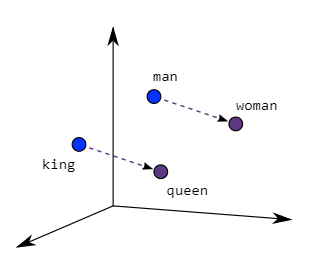
\includegraphics[width=0.5\textwidth]{images/embeddings}
    \caption{Relations between similar word vectors}
    \label{fig:embedding}
\end{figure}
\hfill \break
Logistic regression expects a fixed size input but words and sentences in natural language can be of any size.
Today, this problem is solved by using word embeddings which represent words from our dataset as multidimensional vectors.
Their advantage over some other approaches that were used in the past, such as one-hot vector representation, is that they are able to find relations between words and produce similar vectors for similar words.
The relation between similar words can be seen in figure~\ref{fig:embedding}.
In our approach we used \textbf{word2Vec}~\citep{mikolov2013efficient} embeddings which were trained on the whole training dataset and produced 300-dimensional representations.
Learned word embeddings were then used for calculating the final representation for each training example.
Here we experimented with 2 approaches:
\begin{enumerate}
    \item \label{itm:one} \textbf{Averaging of word embeddings:} summing up each representation in the input sequence and dividing it with the number of words in the sequence
    \item \textbf{TF-IDF averaging:} Term Frequency - Inverse Document Frequency is an algorithm that is used to determine an importance of the given word in the document.
    Importance is represented as a scalar value.
     This scalar value for each word is then multiplied with the word's corresponding representation.
    The final representation is then calculated in the same way as described in approach~\ref{itm:one}.

\end{enumerate}

\subsection{DistilBERT}
The second model we used was DistilBERT~\citep{sanh2020distilbert}.
This model comes from the family of deep learning models called transformers~\citep{vaswani2017attention}.
The main advantage of these types of models is the self-attention mechanism.
Self-attention allows the model to find the importance of each word in a sequence and build more effective contextual representations.
\hfill \break
\hfill \break
DistilBERT is a model similar to the more popular BERT~\citep{devlin2019bert}, but faster and more lightweight while still preserving almost all the capabilities of the larger model.
Because of its features and our limited hardware we decided it would be the best option for representing current SOTA solution in the field of transformers.
Model and tokenizer were trained simultaneously on the whole training set using the implementations from the \textit{HuggingFace} library~\citep{wolf2020huggingfaces}.





\subsection{Chat GPT 3.5 Turbo}
The final model that we used in our research was Chat GPT 3.5 Turbo~\citep{openai2023}.
This model was developed by OpenAI and it aims to generate human like responses based on the provided input text.
We could not perform direct training on this model, but instead we used the provided API to prompt the model to give us the classification result for each example in the test set.
You can see how we formulated our prompt in figure~\ref{fig:chat-gpt-prompt}.

It must be mentioned that there was some manual data cleanup needed after we got the responses from the API, such as explanations behind the given results that were contained in the labels.

\begin{figure}
    \centering
    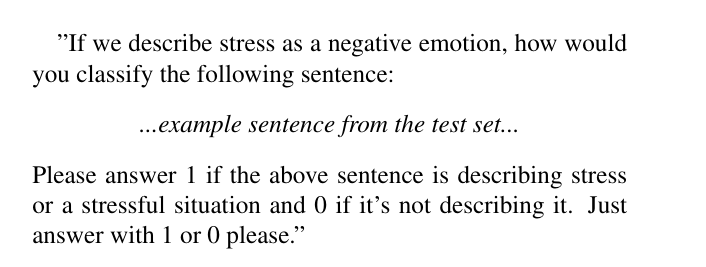
\includegraphics[width=0.5\textwidth]{images/chat-gpt-prompt}
    \caption{Text input for Chat GPT 3.5 Turbo API}
    \label{fig:chat-gpt-prompt}
\end{figure}

\begin{table*}
    \centering
    \caption{Different model results}
    \label{tab:model-results}
    \begin{center}
        \begin{tabular}{|l|c|c|c|}
            \hline
            \textbf{Model} & \textbf{P} & \textbf{R} & \textbf{F1} \\ \hline
            LR + averaged word2Vec embeddings & 0.6441 & 0.7995 & 0.7134 \\ \hline
            LR + TF-IDF averaged word2Vec embeddings & 0.6859 & 0.8049 & 0.7406 \\ \hline
            DistilBERT & \textbf{0.7105} & 0.7913 & 0.7487 \\ \hline
            Chat GPT 3.5 Turbo & 0.6905 & \textbf{0.9431} & \textbf{0.7972} \\ \hline
        \end{tabular}
    \end{center}
\end{table*}

\section{Results}

The results of our four different models are present in table~\ref{tab:model-results}.
We can see that our logistic regression (LR) model with basic word embedding averaging performed the worst, what was expected given its simplicity.
This simple model, however, performs much better when we introduce TF-IDF averaging.
\subsection{LR(TF-IDF averaging) vs DistilBERT}
LR model with TF-IDF averaging performed very similarly to the DistilBERT approach.
Transformers are currently SOTA approach in NLP and we expect them to perform much better than the simpler models.
However, classifying stress, using this pretty clean dataset, is not a particularly hard task and our logistic regression model deals very well with the problem, which is also what authors of the original dataset pointed out.
\hfill \break
\hfill \break
Here we compared only the results of the two models not taking into account the cost of the more complex model.
Training of the DistilBERT model took longer and required more hardware just to get similar results.
This leads us to the conclusion that sometimes the solution to the problem could be a simple model without the need for more complex and expensive solutions.
\\

\begin{figure}
    \centering
    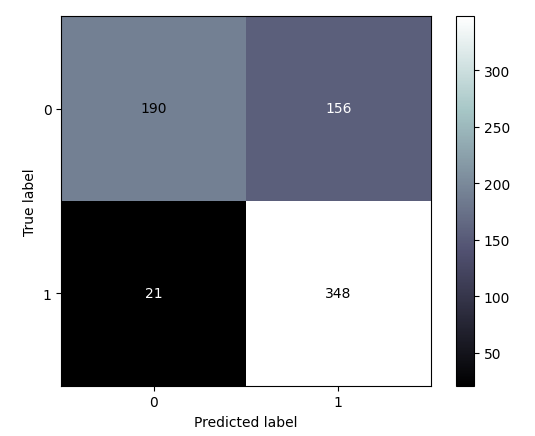
\includegraphics[width=0.5\textwidth]{images/conf-matrix-chatgpt}
    \caption{Confusion matrix for Chat GPT 3.5 Turbo. 0 represents data labeled not stressed while 1 represents data labeled stressed.}
    \label{fig:chat-gpt-conf-matrix}
\end{figure}

\begin{figure}
    \centering
    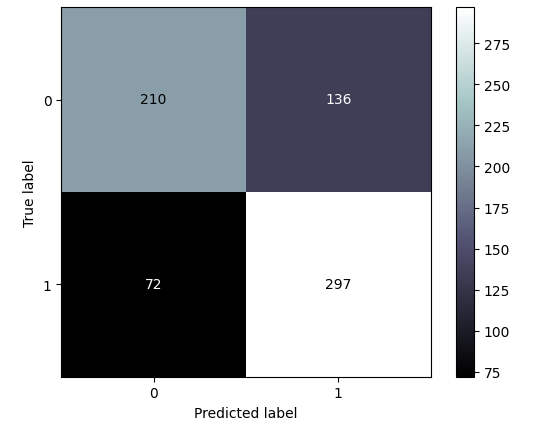
\includegraphics[width=0.5\textwidth]{images/conf-matrix-logreg}
    \caption{Confusion matrix for LR with TF-IDF averaging.}
    \label{fig:logreg-conf-matrix}
\end{figure}


\subsection{DistilBERT vs Chat GPT}
In our two transformer approaches Chat GPT showed much better results.
What shows the true power of this transformer model is that, even though it was not strictly trained on the training data, it managed to outperform DistilBERT model.
As we can see in figure~\ref{fig:chat-gpt-conf-matrix} this model managed to have an extremely low number of false negative (FN) predictions.
In certain cases we would want to prefer this behaviour where not detecting stress represents a big problem.

The downside of this approach is the cost behind it.
Chat GPT API is a paid service and if we want to use this approach in for stress detection this might not be the best option if our budget is limited.

\subsection{LR (TF-IDF) vs Chat GPT}
We can see that Chat GPT performed better than our LR model when we compare their F1 scores.
The change comes primarily from the higher recall score which Chat GPT manages to achieve (less false negative examples).
While we can look at the scores by themselves and conclude that Chat GPT is a better model for the given task, this approach does not take into account the cost of the model.

Our simpler LR model achieves comparable results to the SOTA solution and we claim that it is the optimal approach for solving stress classification problem from the given dataset.
Model is easy to learn and could even get better results if it was trained on the dataset which contained examples with higher agreement factor, as it was shown from the authors of the dataset.

If we have more resources and a bigger budget, Chat GPT with its powerful API service could be a better choice, mainly because it rarely does not detect stress which could definitely help in certain situations.
\section{Conclusion}

In this paper we looked at different approaches for detecting stress from the Dreaddit dataset.
We continued our research on findings of the authors and tried to find out if more complex models and solutions gave better results.
\hfill \break
\hfill \break
We believe that the simple model solves this problem well enough and that more complex and expensive transformer solutions are not worth the extra cost.
In some rare cases, where not detecting stress could pose a problem, we can suggest trying the Chat GPT API service if the demand is not high and the budget is not limited.
Transformers may be a better option if we just look at their capabilities, but at what cost?
Sometimes the simpler solution gets the job done and we should stick to it.

\bibliographystyle{tar2023}
\bibliography{tar2023}

\end{document}

